% Generated by Listas/make_statements.py from pratica-lecture-08.md, item 6. Do not edit.
\textbf{Source.} Gibbons (1992), \emph{Game Theory for Applied Economists}, §4.2 Problems, Problem 4.4, p.~248 {[}PDF p.~254{]}. Reproduced verbatim. Answer: none in the book.



\begin{quote}

4.4. Describe all the pure-strategy pooling and separating perfect Bayesian equilibria in the following signaling games.



\pandocbounded{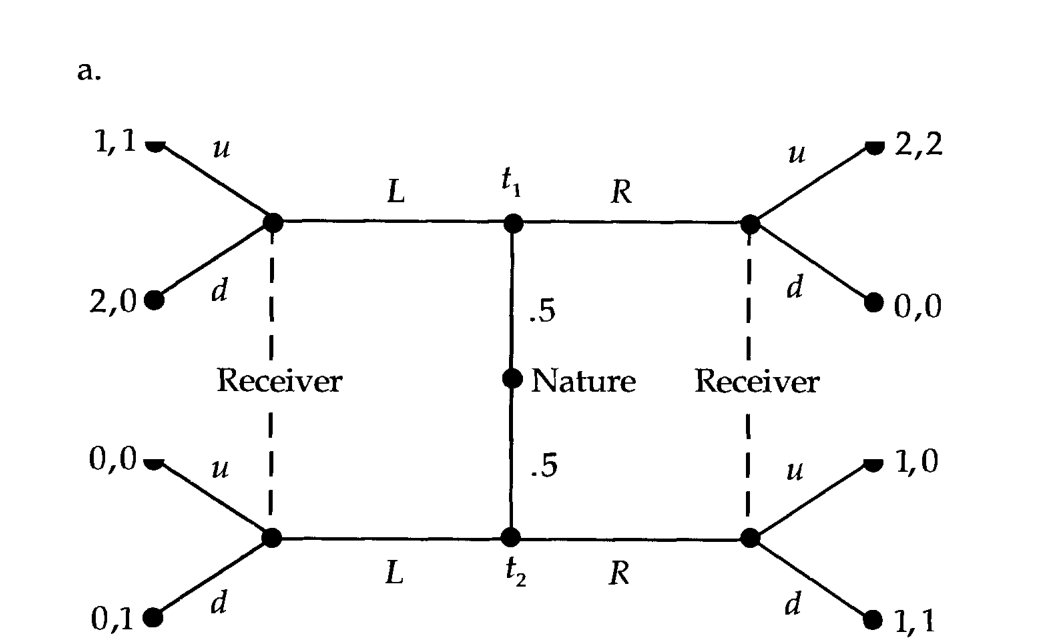
\includegraphics[keepaspectratio,alt={Problem 4.4, game a}]{../figures/gibbons-4-4a.png}}



\pandocbounded{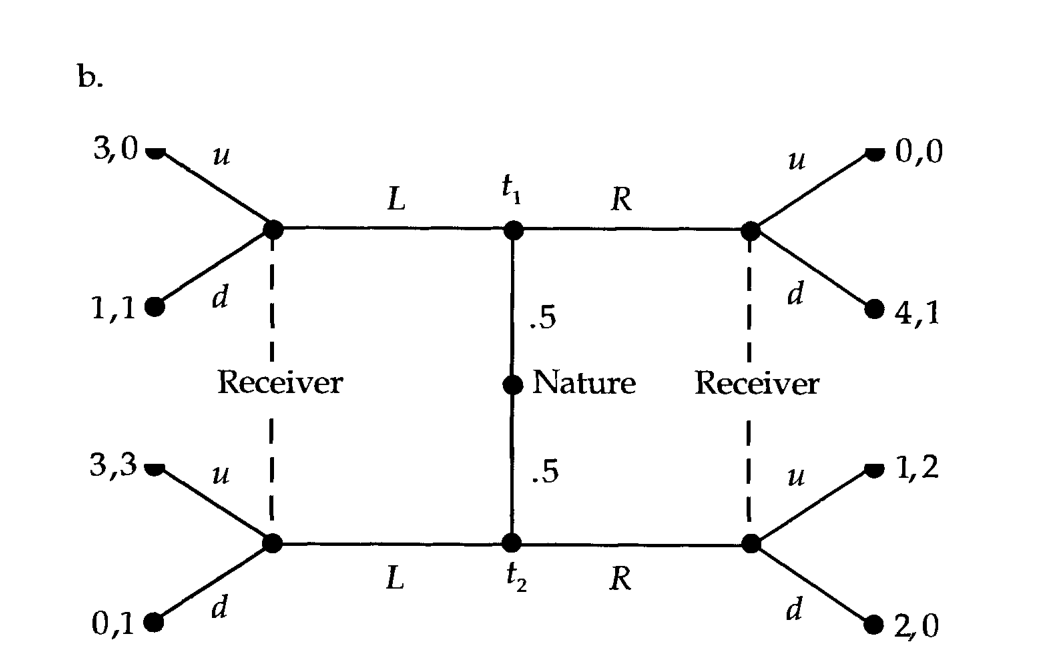
\includegraphics[keepaspectratio,alt={Problem 4.4, game b}]{../figures/gibbons-4-4b.png}}

\end{quote}

